\section{Overall Description}

\subsection{Product perspective}
eMall helps on the first hand to manage to limit the carbon footprint caused by our urban and sub-urban mobility needs,
providing a way to introduce minimal interference and constraints on the owner EV daily schedule;
on the other hand the eMall helps the CPOs to manage remotely their EVCP.
\vspace{1cm}
\subsubsection{Entity diagram}
The UML entity diagram below represents a conceptual, high-level model of
the software to be. Given its nature, it may model objects that will not
be represented in the actual system that will be developed. At this
level, it not include any references to methods and other low-level
details, those will be detailed during the design phase.
\begin{figure}[H]
      \centering
      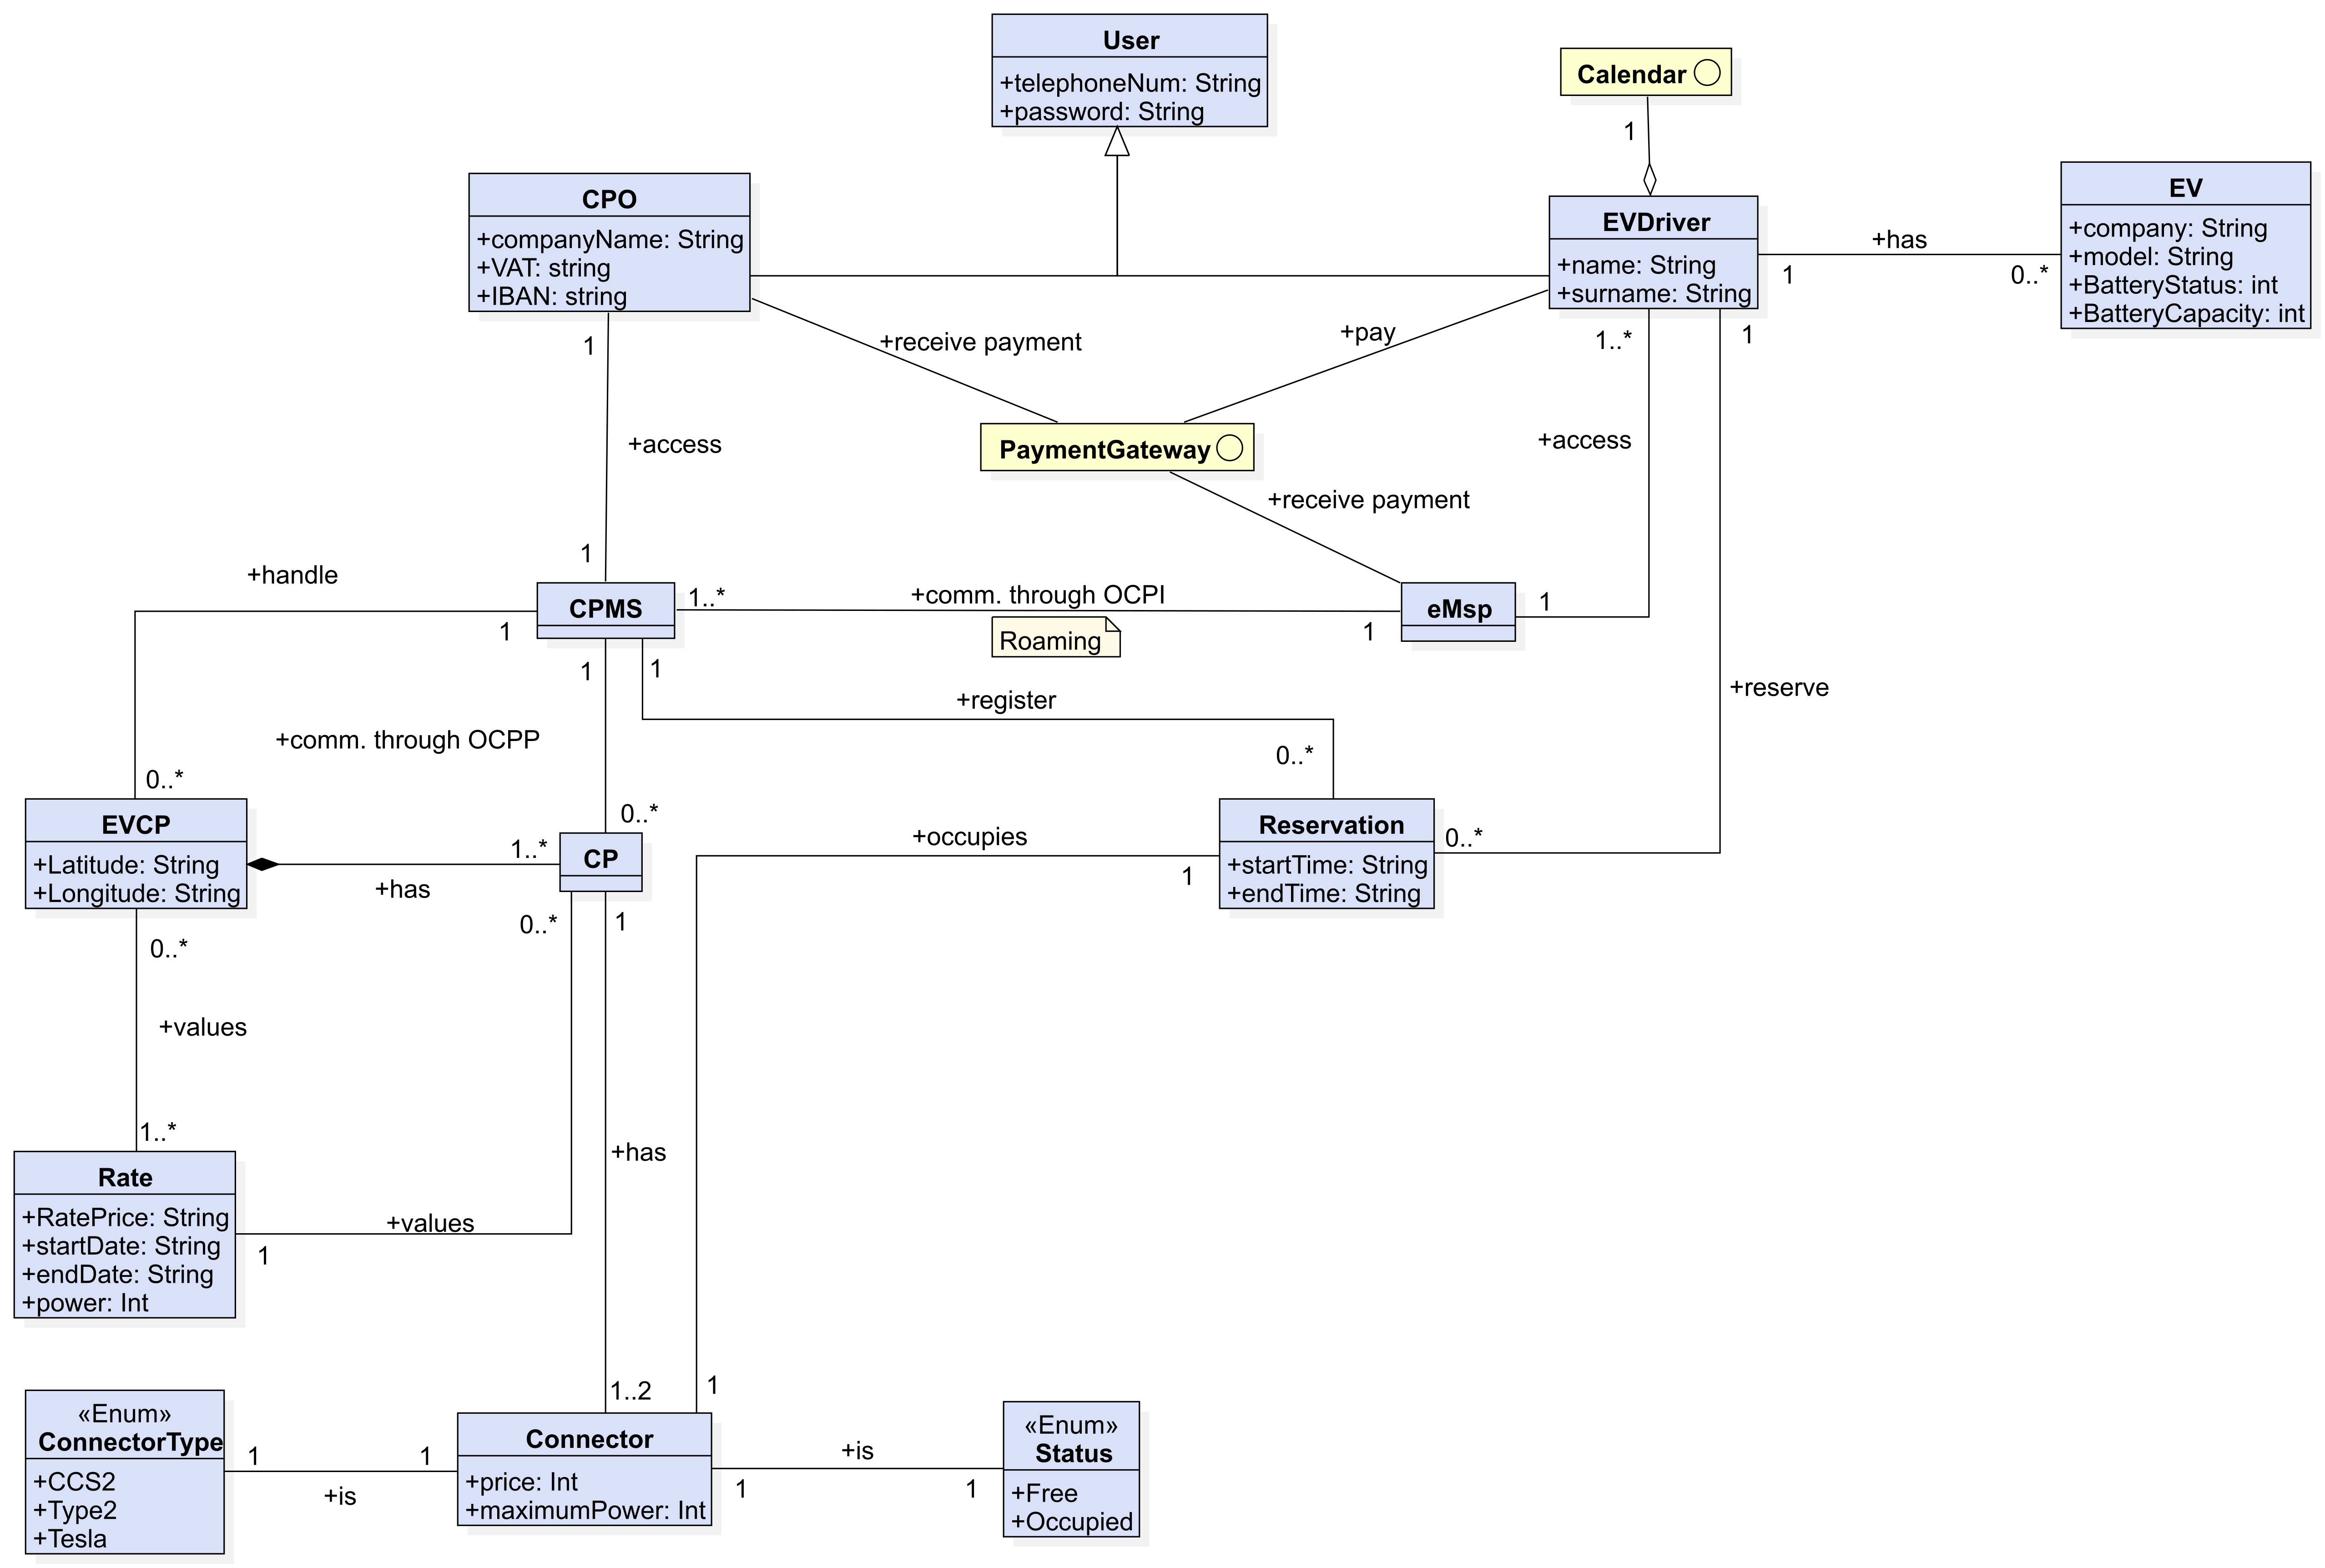
\includegraphics[scale=0.4]{src/domain_UML.png}
\end{figure} \vspace{1cm}

\subsubsection{State diagrams}
In the paragraphs below, a representation of the behavior of the main conceptual
components of the system. The focus is on how these components respond to
external influences and modify accordingly their states. For this purpose,
some UML State Charts are proposed:

\begin{figure}[H]
      \centering
      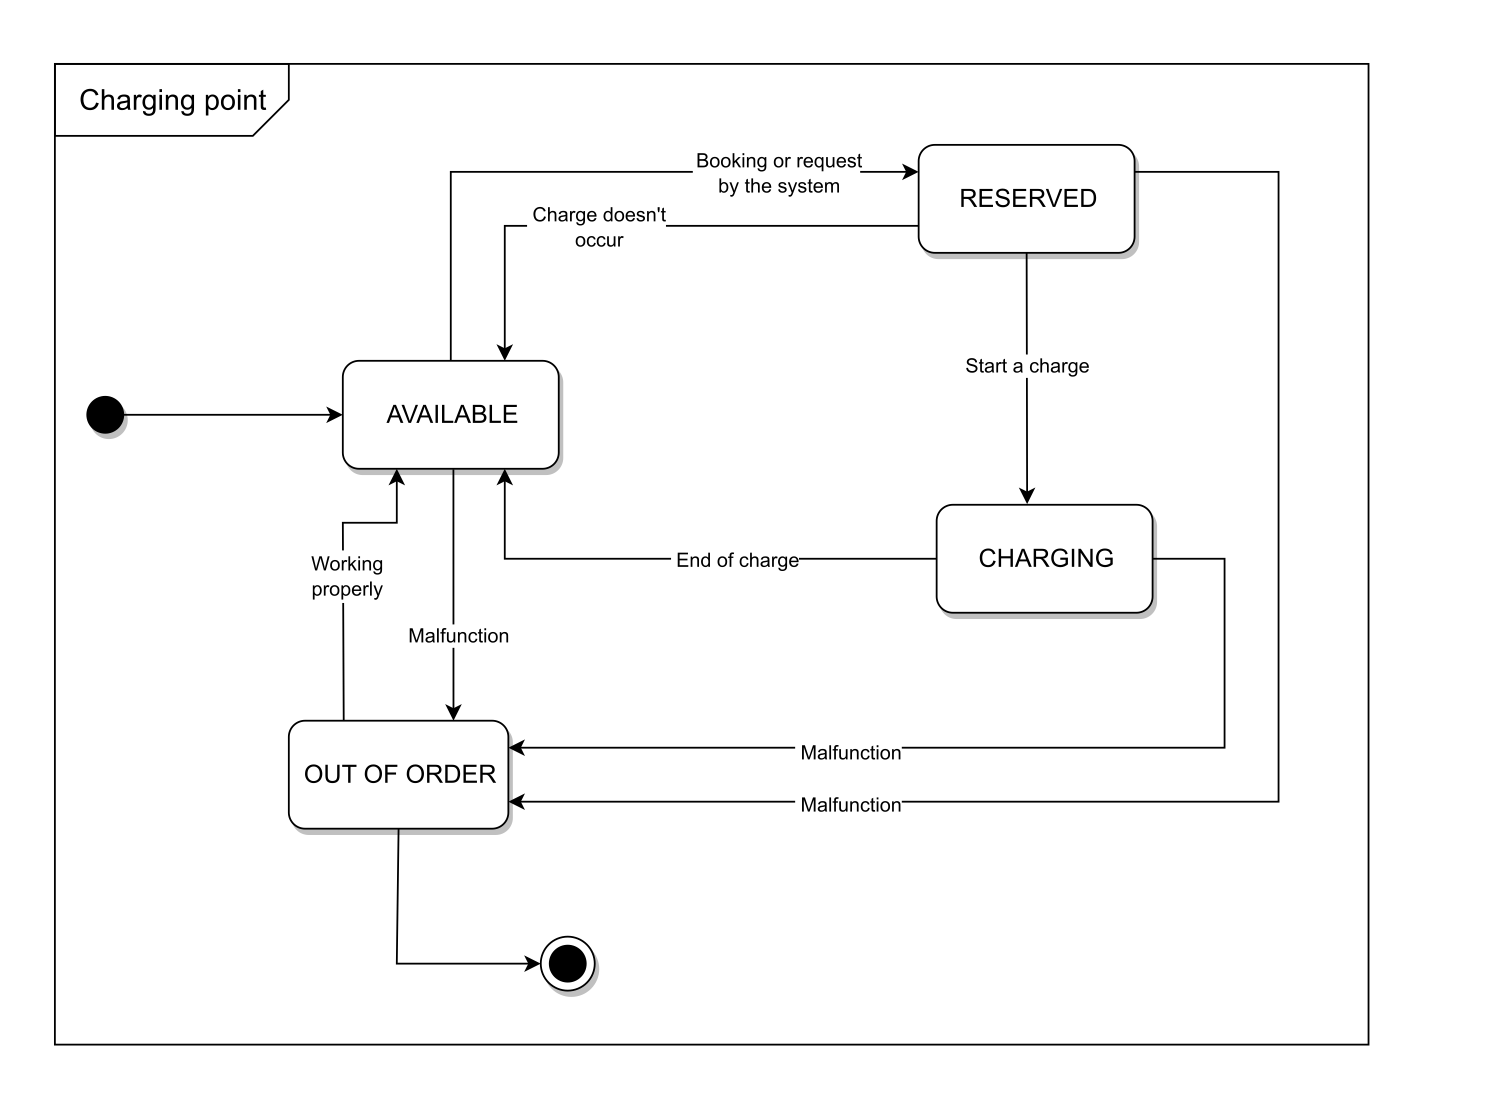
\includegraphics[scale=0.2]{src/state_diagram/cp.png}
\end{figure} \vspace{1cm}
\begin{figure}[H]
      \centering
      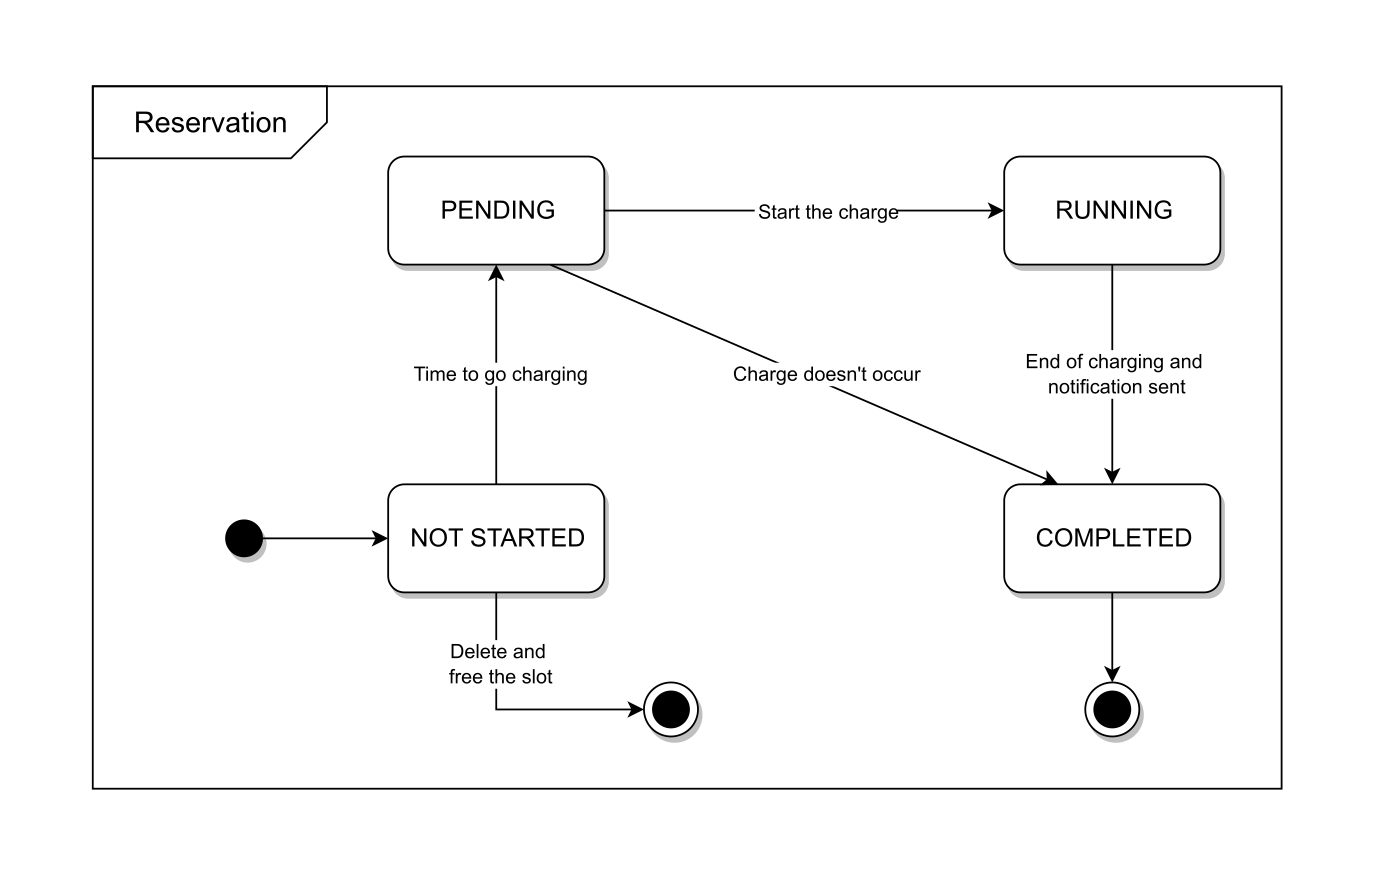
\includegraphics[scale=0.2]{src/state_diagram/transaction.png}
\end{figure} \vspace{1cm}

\subsubsection{Scenarios}
\begin{enumerate}[label=\textbf{\Alph*}.]
      \item \textbf{Registration} \\
            Einar is a driver of an electric vehicle that uses every day to go to his
            office. He decided to download the eMall app because he heard by a friend
            of him that he can discover all the charging points in the entire world,
            booking one, starting a charge and pay for the charge, entirely through
            the app. After having downloaded it, launches the app for the first time
            and select sign in button to register into the system. He provides all
            the personal data required to access in the system and accept to personalize
            his experience by selecting his car from a provided list of all the EVs.
            He submits his data and the system asks him to verify his account through email or phone number.
      \item \textbf{Book a charge} \\
            Edvar has the necessity to go shopping in the next days at the blue and yellow furniture retailer of the city. Knowing
            that shopping will take some time he wants to find and book a EVCP nearby the shopping centre to charge his EV that uses every day.
            In the home of the app he filters the results on the location of the mall and the day he wants to go.
            After submitting the form, the home page change according to his information and displays
            a map of the selected zone with the available charging stations to book. He discovers that there is one available
            really close from the shopping centre. He selects the marker of the EVCP and are displyed the information about the CPO,
            the types of CP, the availability at the actual moment of the research, the availability of them for the filtered date,
            the charging power at which the connector operates and the cost for recharging 1 kWh.
            To book the charge he selects one connector that is available and indicate when he wants to start the charge
            and when to finish. The app, because Edvar accepted to insert his EV model, knows how much time is needed to charge his car so suggested
            the optimal time to book for a complete charge from 10\% to 100\%.
            He can accept the suggested book range or override the suggestion and modify the range at his willing inside the
            availability of the connector. He then confirms the booking of the charge and see the reservation on the reservations' tab.
      \item \textbf{Manage a charge} \\
            Anne plans a long trip from Oslo to Stockholm to do with her brand new EV.
            Considering the suggested time by the app to do a full charge on her EV, she books a three hour charge through the eMall
            app at her trusted charging station with high power connectors.
            When she arrives at the CP station she parks in a free slot with the booked connector. Through the app she selects
            the reservation in the reservations' tab and starts the charge inside the app. The connector socket is unlocked and
            the charge can start by plugging the connector on the EV. Meanwhile waiting for the complete charge, Anne goes for a walk
            because she feels relaxed to control at any time the status and the remaining time of the charge with the app. When the charge
            is completed, as expected before the three hours, Anne is already back from the walk and a notification about the end of the charge
            appears on Anne's phone, she disconnects the connector and gets back home to prepare the luggages for the trip. She doesn't worry about
            the payment because is executed in background with the payment method that she indicates before the booking operation.
      \item \textbf{Charging point status} \\
            Erling is the owner of a restaurant and installed two charging columns in the parking slot in front of the restaurant because
            he wants to acquire good clients that can stop for charging the EV and have a meal at the restaurant. To make the CP accessible to the largest
            possible public he subscribes to the eMall-business for CPOs because he is interested in a service that permits to add and manage CPs and make
            the CPs visible by EV drivers in the eMall app. After submitting the registration by providing essential information about the the company, including
            VAT number of the restaurant and IBAN bank account to get payments from the driver he waits for the approval to be inserted into the app.
            When the approval arrives Erling inserts the charging point of the restaurant by specifying the number of sockets by type, the amount of power supplied by
            each socket and the API to connect the charging columns to the dashboard. With the dashboard he can visualize how many vechicles are charging in real time
            and for each charging vehicle the amount of power absorbed and the time left to the end of the charge. He can visualize the import that gets from each
            charge, decide the price for a charge and add special promotions to the charge to win the loyalty of the existing clients or acquire new clients.
      \item \textbf{Charging point management} \\
            Grethe, admin of a CPO using the CPMS function of eMall from the early days, receives an mail from the CPMS about a malfunction involving one of her CPs.
            She enters the CPMS and directly from the dashboard she modifies the CP status to "in maintenance".
            She is sure that the CP under mantainance now results as unvailable for every user trying to book it until she modifies back the status to "available".
            Then verifies the status of the others CP controlling that they work as intended.
\end{enumerate}

\subsection{Product functions todo:expand this description a little}
As described above in this document, the major functions offered by our system to main actors are:\\
\begin{itemize}
      \item \textbf{EV driver's functions. The system allows to:}
            \begin{itemize}
                  \item search in map
                  \item view your current position
                  \item indicate time interval of charging
                  \item have suggestion on when to charge based on daily schedule and special offers
                  \item specify the charging point in which you want charge
                  \item book a charge
            \end{itemize}
\end{itemize}
\begin{itemize}
      \item \textbf{CPO's functions. The system allows to:}
            \begin{itemize}
                  \item monitor status of CPs
                  \item add, modify and delete CP
                  \item retrieve price of energy from the available DSOs
                  \item manually change status of a CP
                  \item view reservations on their CPs
                  \item managing charging point
            \end{itemize}
\end{itemize}


\subsection{User characteristics todo:insert background of actors}
It is possible to distinguish two different types of actors who use the system:
\begin{enumerate}
      \item EV's driver: someone who wants to book a charge. EV's driver wants to book remotely
            avoids interference in his daily schedule, be notified when his/her reservation
            is going to start and end, monitor charging process.
      \item CPO: someone who wants to manage efficiently his/her EVCP, make statistics on live and historical details on the EVCP,
            to acquire information on the current price of energy offer by DSOs and to decide in an automated way
            where to get energy for charging.
\end{enumerate}


\subsection{Assumptions, dependencies and constraints}
\subsubsection*{Domain Assumptions}
\begin{table}[H]
      \begin{tabularx}{\textwidth}{cX}
            \toprule
            \textbf{D1} & An EV driver arrives at the charging station at a time close to its reservation starting time \\
            \textbf{D2} & An EV driver leaves the charging station when the charge is finished                          \\
            \textbf{D3} & An EV driver doesn't occupy an already booked charging spot                                   \\
            \textbf{D4} & The accurate location of an EV driver is known by GPS                                         \\
            \textbf{D5} & An EV driver provides correct information when registering                                    \\
            \textbf{D6} & A CPO provides correct data of its EVSEs when registering                                     \\
            \textbf{D7} & At least one DSO can always provide energy to the CPOs                                        \\
            \textbf{D8} & An user that books a charge has an electric vehicle to charge                                 \\
            \textbf{D9} & An user that books a charge is always reliable   \\
            \textbf{D9} & The external APIs are always reliable and working   
            \\\bottomrule
      \end{tabularx}
\end{table}
\subsubsection*{Dependencies}
\begin{itemize}
      \item The system requires access to a third party maps API.
      \item The system will use the GPS of the driver's computer or smartphone
      \item The system will require internet connection to interact with all the users
      \item The system will use an external API to retrieve the prices of energy by the available DSOs
      \item The system will use an external API to retrieve the EV battery status and a list of EV available on the market
      \item The system will use an external API to retrieve information about the status of an energy storage system and solar panels production in the EVCP
      \item The system will use an external API to retrieve data or send data to the CPs
      \item The system will use an external API to access the calendar of the usery
      \item The system will use a payment gateway to perform payment operations
      \item The system will use an external API to send push notification to the drivers
      \item The system needs a third party API in order to send SMS to customers phones.
\end{itemize}
